\documentclass[12pt,a4paper]{monografia}
\usepackage[english,brazilian]{babel}
\usepackage[utf8]{inputenc}
\usepackage[T1]{fontenc}
\usepackage{amsmath,amsthm,amsfonts,amssymb,textcomp}
%\usepackage{latexsym}
\usepackage[]{graphicx}
\graphicspath{{figuras}}
\usepackage{subfigure}
\usepackage{float}
\usepackage{longtable}
\usepackage{color}
\usepackage{epstopdf}
\usepackage{pdflscape}
\usepackage[comma,authoryear]{natbib}
\usepackage{hyperref}
\usepackage[nonumberlist]{glossaries}
%\usepackage[alf]{abntcite}
\bibliographystyle{apalike}

\newcommand{\PE}{Perkin-Elmer}
\newcommand{\BC}{Boller \& Chivens}

\makeglossaries



\newglossaryentry{Offset}{name={Offset}, description={Diferença entre a posição obtida pela redução da observação e a posição dada pela efeméride}}
\newglossaryentry{OPD}{name={OPD}, description={Observatório do Pico dos Dias - Brasópolis, MG}}
\newglossaryentry{LNA}{name={LNA}, description={Laboratório Nacional de Astrofísica - Itajubá, MG}}
\newglossaryentry{OHP}{name={OHP}, description={Observatoire Haute Provence - Saint-Michel-l'Observatoire, França}}
\newglossaryentry{RA}{name={RA}, description={Sigla para Ascensão Reta ($ \alpha $)}}
\newglossaryentry{DEC}{name={DEC}, description={Sigla para Declinação ($ \delta $)}}
\newglossaryentry{Anomalia Verdadeira}{name={Anomalia Verdadeira}, description={Ângulo formado entre o Periastro e a posição instantânea do objeto na órbita centrado no planeta e contada na direção do movimento orbital}}

\begin{document}
\doutorado

\titulo{Aplicações Astrométricas e Fotométricas para o Estudo do Sistema Solar Exterior}
\autor{Altair Ramos Gomes Júnior}
\ultimonome{Gomes Júnior}
\nome{Altair Ramos}
\orientador{Marcelo Assafin}
\ttorientador{Professor Doutor}
\curso{Astronomia}
\instituicao{Universidade Federal do Rio de Janeiro}
\sigla{UFRJ}
\unidadeacademica{Centro de Ciências Matemáticas e da Natureza\\Observatório do Valongo}
\ano{2015}
\data{Junho de 2015}
\cidade{Rio de Janeiro}
\examinadorum{Primeira Pessoa}
\examinadordois{Segunda Pessoa}
\examinadortres{Terceira Pessoa}
\examinadorquatro{Quarta Pessoa}
\ttexaminadorum{Doutor}
\ttexaminadordois{Doutor}
\ttexaminadortres{bacharel}
\ttexaminadorquatro{licenciado}
\CDU{521.9}
\areas{Astrometria}
\npaginas{160}

\maketitle

%\begin{agradecimento}{Dedicatória}
%\indent \indent Agradeço à minha mãe Adelma e meu pai Altair por todo o apoio emocional e financeiro durante a minha trajetória acadêmica. Ao meu irmão, que sempre me incentivou, aos meus amigos e colegas pela troca de experiências.\\
%\indent À minha tia Maria do Carmo pelo auxílio dado para minha permanência no Rio de Janeiro, sem a qual não teria sido possível ficar no curso.\\
%\indent Ao meu orientador Marcelo Assafin por ter me aceito como aluno e me dado a oportunidade de trabalhar com as empolgantes áreas de Astrometria e Sistema Solar e por sua paciência ao me ensinar e me atualizar sobre o campo de trabalho.
%\end{agradecimento}

%\newpage
%\begin{epigrafe}
%"Queremos ter certezas e não dúvidas, resultados e não experiências, mas nem mesmo percebemos que as certezas só podem surgir através das dúvidas e os resultados somente através das experiências."\\
%\hfill Carl Gustav Jung
%\end{epigrafe}

\resumo{Resumo}
\indent \indent O estudo da estrutura e evolução do Sistema Solar tem muita importância atualmente, por exemplo, na compreensão dos mecanismos de formação dos planetas de outras estrelas (exoplanetas), trazendo em seus desdobramentos valiosas informações quanto a viabilidade de formação de ambientes que comportem vida.\\
\indent Praticamente cada satélite é um problema particular de Mecânica Celeste. Dessa forma, a observação de seus movimentos é muito útil por razões teóricas. A preparação e realização de missões espaciais para alguns planetas, e mesmo alguns satélites, como Titã de Saturno ou os Galileanos de Júpiter, requer observações frequentes e posições muito acuradas de todos os satélites do sistema planetário visitado.\\
\indent Os satélites irregulares de planetas gigantes, principalmente de Júpiter e de Saturno, são substancialmente menores do que os satélites regulares e possuem órbitas mais distantes, excêntricas, inclinadas e, na maioria dos casos, retrógradas. Explicar a existência dos satélites irregulares dos planetas gigantes é um estudo interessante em dinâmica orbital.\\
\indent É amplamente aceito que eles, devido à configuração orbital, foram capturados por seus planetas. Porém, ainda não são certos a origem e o método de captura desses objetos embora as teorias mais prováveis sejam a de arrasto gasoso durante a formação do Sistema Solar e a captura de três corpos.\\
\indent A maioria dos satélites formam famílias com características orbitais semelhantes sugerindo uma evolução dada por colisões. A compreensão desses mecanismos nos fará entender melhor o nosso próprio sistema solar e, possivelmente, de sistemas extra-solares.\\
\indent Com o pacote astrométrico PRAIA o tempo empregado na redução de grandes quantidades de imagens foi diminuído significativamente. Os objetivos científicos dos nossos programas observacionais agora tem sido atingidos em curtíssimo prazo, em consonância com a atual demanda astronômica e astrofísica de nossa área.\\
\indent Em uma base de dados com mais de 100 mil imagens obtidas entre 1992 e 2012 no telescópios de 1.2m do Observatoire de Haute Province, França, e nos telescópios \PE, \BC{} e Zeiss no Observatório do Pico dos Dias, mais de 4 mil contem satélites irregulares de Júpiter e Saturno. Reduzir essa grande quantidade de observações com precisão só foi possível com a utilização do PRAIA. Como é possível ver nos resultados obtidos, os offsets de posição refletem o erro natural da astrometria e o erro das efemérides dos satélites mais fracos, e sugerem que podemos efetivamente contribuir para que novas integrações numéricas forneçam posições mais precisas. Essas novas efemérides irão permitir que ocultações estelares por esses objetos possam ser preditas com maior precisão. A observações dessas ocultações permitirão um maior conhecimento das propriedades físicas dos satélites.

\par
\vspace{1em}
\noindent\textbf{Palavras-chave:} Astrometria, Satélites Irregulares de Júpiter, Satélites Irregulares de Saturno


\tableofcontents % para gerar o sumário
\thispagestyle{empty} % para que a pagina não seja enumerada
%\listoffigures % cria a lista de figuras
%\thispagestyle{empty}
%\listoftables % cria a lista de tabela
%\thispagestyle{empty}

\pagestyle{ruledheader}

\chapter{Introdução}
\label{Cap: intro}

\indent \indent O estudo de objetos como TNOs, Centauros e Satélites Irregulares (remanescentes relativamente inalterados da formação do sistema solar) nos ajudam a compreender a formação e evolução do Sistema Solar. Atualmente, é aceito que TNOs e Centauros tenham sido formados nas partes mais internas do sistema solar. Eles teriam então sido colocados em suas posições atuais devido a troca de momento angular entre os planetas e planetésimos quando da migração dos planetas gigantes. A evolução se deu de tal forma que a passagem dos planetesimais e planetas por zonas de ressonância de movimento médio redefiniu as órbitas desses corpos \citep{Tsiganis2005}.\\
\indent Sabe-se que poucas sondas espaciais foram enviados para estudar o Sistema Solar Externo e que a quantidade de objetos estudados é muito pequena. Por isso, ainda hoje, as observações de solo tem se mostrado de grande importância.\\
\indent Os sistemas de Júpiter e Saturno já foram pelas Voyager I e II, Galileu (Júpiter) e Cassini (Saturno), porém apenas Saturno continua sendo investigado por uma sonda. Porém as sondas observaram apenas os planetas, os anéis e satélites mais internos. Os satélites externos, que acredita-se ser oriundo de capturas ou foram pouco observados (como Phoebe) ou simplesmente não foram observados.\\
\indent Já no caso de Urano e Netuno, nenhuma sonda exclusiva foi enviada, apenas as Voyagers I e II os visitaram, mas não permaneceram nos sistemas. A sonda New Horizons visitará Plutão em 2015 e obterá parâmetros físicos para Plutão e seus satélites (primeira visita por sonda a um satélite do cinturão de Kuiper), porém será uma passagem rápida e o acompanhamento da evolução do sistema, incluindo a evolução da atmosfera de Plutão se dará por observações de solo.\\
\indent A quantidade de objetos descobertos além da órbita de Saturno tem aumentado muito desde o fim do século passado. Como são raras as oportunidades em que uma sonda se aproxima desses objetos, a obtenção de suas características físicas ficam a cargo de observações de solo ou de
telescópios espaciais.\\
\indent Um método que tem se mostrado eficiente para a obtenção desses parâmetros é o métodode ocultações estelares, que proporciona medidas tão precisas que são apenas superadas por medidas oriundas de sondas.

\chapter{Ocultações}
\label{Cap: observacoes}

\section{Ceres}
\label{Sec: Ceres}

\indent \indent Apesar de Ceres não ser um objeto do sistema solar exterior, ele é o único planeta-anão no sistema solar interno e, por isso, é um objeto de grande importância e seu estudo pode ter grande impacto na formação e evolução do sistema solar. Na verdade, foi proposto que a origem de Ceres pode ser como um objeto transnetuniano \citep{McKinnon2012}, espalhado posteriormente para o cinturão principal de asteroides devido à migração dos planetas gigantes predito pelo Modelo de Nice \citep{Gomes2005}. Mesmo que ele tenha sido formado próximo à sua localização atual, a história dinâmica do sistema solar deve ter deixado sua assinatura em Ceres.\\
\indent Contendo aproximadamente um quinto de toda a massa do cinturão de asteroides, espera-se que Ceres esteja em equilíbrio gravitacional e seja, portanto, um elipsóide Maclaurin ou Jacobi. De fato, observações diretas de Ceres com a utilização de ótica adaptativa indica que ele é um esferóide achatado nos pólos \citep{Drummond2014}. O conhecimento preciso de seu tamanho e forma é extrema importância para modelos de densidade, estrutura interna e diferenciação.

\begin{figure}
\begin{centering}
\subfigure[Ocultação de 2010]{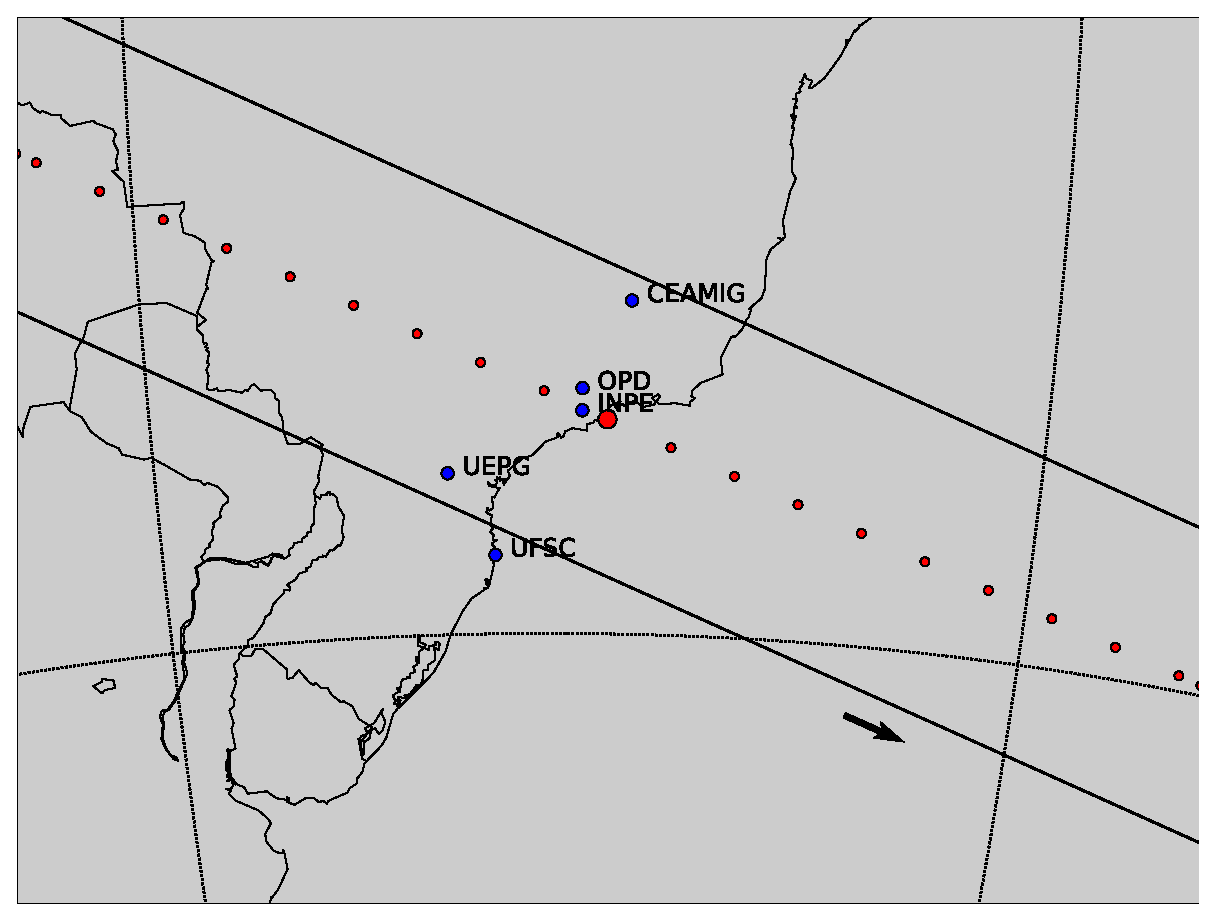
\includegraphics[scale=0.39]{figuras/Ceres_2010.eps}\label{Fig: Ceres-map-2010}}
\subfigure[Ocultação de 2013]{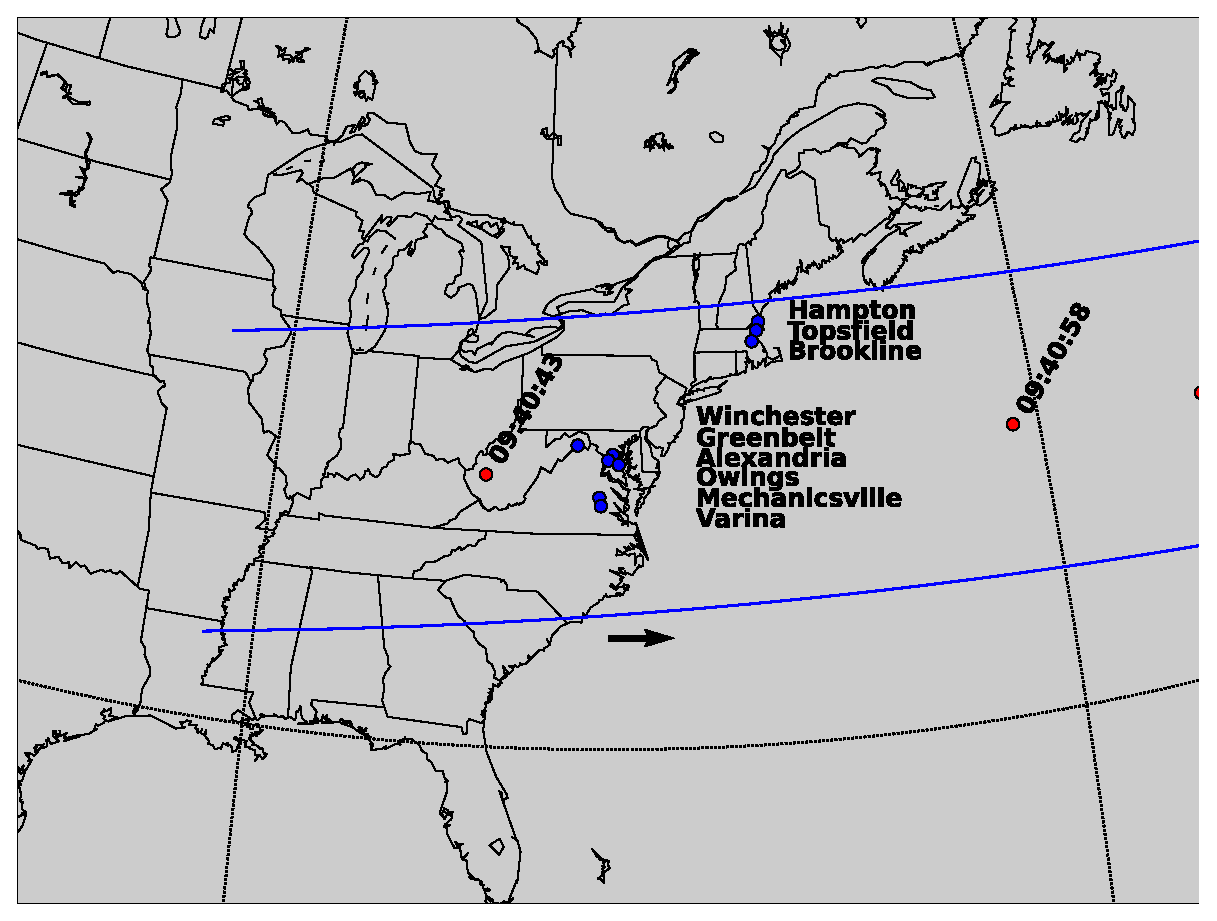
\includegraphics[scale=0.39]{figuras/Ceres_2013-zoom.eps}\label{Fig: Ceres-map-2013}}
\caption{Reconstrução pós-ocultação do caminho da sombra de Ceres na Terra para os eventos de 17 de Agosto de 2010 (a) e 25 de Outubro de 2013 (b). Os pontos em azul são os sítios que observaram os eventos. a) O ponto grande vermelho é a máxima aproximação geocêntrica às 22:40:25 UT. Os pequenos representam o centro da sombra separados por um minuto. b) Visão superior da ocultação sobre os sítios que observaram o evento de 25 de Outubro de 2013. Os pontos vermelhos são os centros da sombra separados por 15 segundos. Nos dois eventos a sombra se move da esquerda pra direita.
\label{Fig: Ceres-map}}
\end{centering}
\end{figure}

\begin{figure}
\begin{centering}
\subfigure[Ocultação de 2010]{\includegraphics[scale=0.35]{figuras/Ceres_2010_sphere.eps}\label{Fig: Ceres-limb-2010} }
\subfigure[Ocultação de 2013]{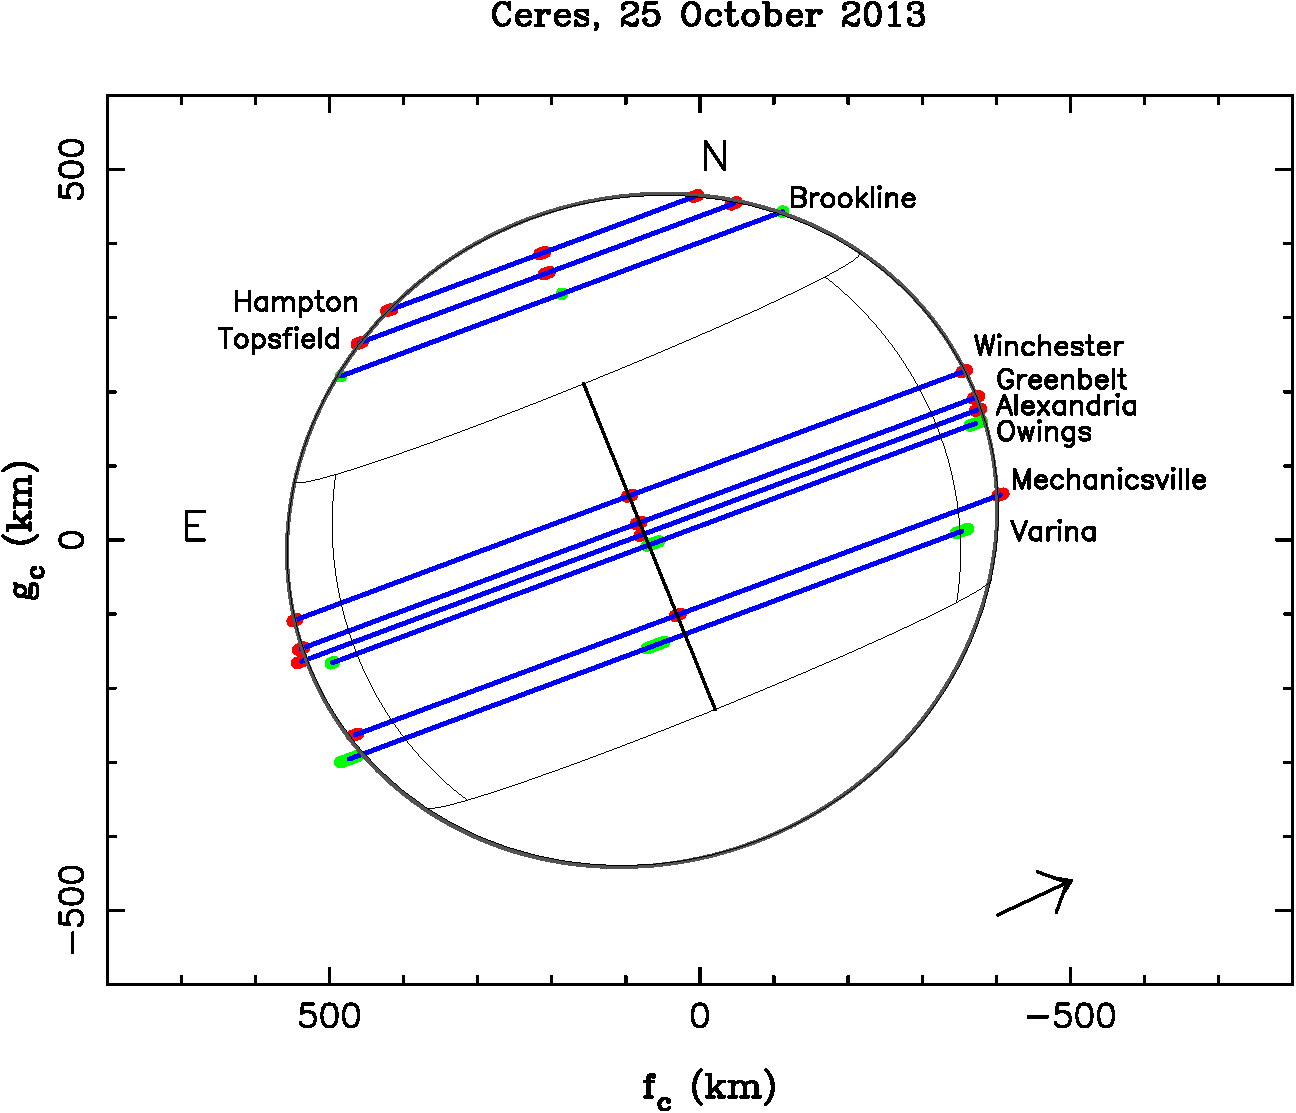
\includegraphics[scale=0.35]{figuras/Ceres_2013_sphere.pdf}\label{Fig: Ceres-limb-2013} }
\caption{Melhores ajustes elípticos para as cordas das ocultações de 2010 e 2013. As setas indicam a direção de movimento, as linhas azuis são as cordas observadas, os segmentos vermelhos são as barras de erro dos ingressos, egressos e centro da ocultação em $1\sigma$. A linha verde em (a) é uma corda negativa. Os instantes marcados em verde em (b) não foram utilizados para o ajuste como descrito no texto.
\label{Fig: Ceres-limb}}
\end{centering}
\end{figure}

\section{Satélites Irregulares}
\label{Sec: Irregulares}

\section{TNOs}
\label{Sec: TNOs}

\chapter{Astrometria de Netuno e Tritão}
\label{Cap: Netuno}



\glsaddall
\printglossary


\bibliography{Referencias}


\end{document}
